\documentclass[11pt,letterpaper]{article}
\usepackage[T1]{fontenc}
\usepackage[utf8]{inputenc}
\usepackage{lmodern}
\usepackage[margin=1in]{geometry}
\usepackage{amsmath,amssymb,amsthm,mathtools}
\usepackage{microtype,booktabs,longtable,tabularx,array}
\usepackage{enumitem,xcolor,graphicx}
\usepackage{listings,xurl,hyperref,bookmark}
\usepackage{fancyhdr}
\definecolor{ink}{HTML}{15324F}
\definecolor{accent}{HTML}{14666B}
\definecolor{muted}{HTML}{5A6570}
\hypersetup{colorlinks=true,linkcolor=ink,citecolor=accent,urlcolor=accent,
 pdftitle={Unknot Recognition by Structural Certificates and Compressed Chain Complexes},
 pdfauthor={ProveIt research continuation}}
\pagestyle{fancy}\fancyhf{}
\fancyhead[L]{\small\textcolor{muted}{ProveIt: unknot recognition}}
\fancyhead[R]{\small\textcolor{muted}{Structural certificates and compression}}
\fancyfoot[C]{\thepage}
\setlength{\headheight}{14pt}
\setlength{\emergencystretch}{2em}
\setlist{itemsep=3pt,topsep=5pt}
\lstset{basicstyle=\small\ttfamily,breaklines=true,columns=fullflexible,
 frame=single,rulecolor=\color{muted!35},backgroundcolor=\color{muted!3},
 showstringspaces=false,keepspaces=true}
\newtheorem{theorem}{Theorem}[section]
\newtheorem{lemma}[theorem]{Lemma}
\newtheorem{proposition}[theorem]{Proposition}
\newtheorem{corollary}[theorem]{Corollary}
\newtheorem{definition}[theorem]{Definition}
\newtheorem{example}[theorem]{Example}
\newtheorem{remark}[theorem]{Remark}
\newcommand{\F}{\mathbb F_2}
\newcommand{\N}{\mathbb N}
\newcommand{\Z}{\mathbb Z}
\newcommand{\Q}{\mathbb Q}
\newcommand{\Kh}{\operatorname{Kh}}
\newcommand{\rKh}{\widetilde{\operatorname{Kh}}}
\newcommand{\rank}{\operatorname{rank}}
\newcommand{\capthree}{\operatorname{cap}_3}
\newcolumntype{Y}{>{\raggedright\arraybackslash}X}
\newcommand{\code}[1]{\texttt{#1}}
\newcommand{\UNKNOT}{\textup{\textsc{unknot}}}
\newcommand{\KNOTTED}{\textup{\textsc{knotted}}}
\newcommand{\UNKNOWN}{\textup{\textsc{unknown}}}
\newcommand{\pin}{\nolinkurl{4e6fe879e5238ec0b134b6d33fdca0b8c7c1c711}}
\title{\textcolor{ink}{Unknot Recognition by Structural Certificates\newline
and Compressed Chain Complexes}\\[6pt]
\large Exact improvements and a finite-type route towards quasi-polynomial time}
\author{Research continuation for the ProveIt project}
\date{7 October 2026}
\begin{document}
\maketitle
\begin{abstract}
We continue the ProveIt unknot-recognition implementation from a pinned,
fully tested source snapshot. Two complementary improvements are developed.
First, signed Seifert-graph certificates give a linear-time decision procedure
(after validation, in the word-RAM model) on every homogeneous knot diagram and an additional one-sided obstruction
on nonhomogeneous diagrams. Second, a scanning Khovanov complex is represented
as a sum of distinct, explicitly serialized differential components with
multiplicity polynomials. Repeated components are continued once, even when
their virtual multiplicity is exponential. A decision-only specialization
replaces those polynomials by the four-element semiring of nonnegative counts
saturated at three; this preserves the final unreduced rank-two unknot test.
An optional exact suffix-Euler calculation supplies monotone lower bounds on
completed homology rank, sometimes deciding knottedness before closure.

We prove preservation of the represented complex, the saturation theorem,
and a quantitative finite-type bound. If $w$ is the maximum frontier size and
$b$ the maximum connected differential-component size produced after
elimination, the number of stored component types at any stage is at most
$\sum_{s\le b}s^s((w-1)!!)^s2^{s^2 2^{w/2}}$. This yields the specific
$n^{O(\log n)}$ target whenever $b^2 2^{w/2}=O(\log^2 n)$, with no restriction
on the number of repeated copies. The hypothesis is an execution parameter,
not a proved universal property of knot diagrams.

The deliverable includes the implementation, independent certificate replay,
regression tests, randomized comparisons, paired timing data, an unchanged
reference implementation, and integration instructions. Explicit-basis
homology computation can still require exponential time even for
three-strand braids. We do not establish a general quasi-polynomial unknot
recognizer. The new results isolate a concrete mechanism by which a complete
implementation can avoid multiplicity growth, and identify the structural
bounds still needed to turn that mechanism into a general complexity theorem.
\end{abstract}
\clearpage
{\fontsize{9.5}{11}\selectfont\tableofcontents}
\newpage

\section{Results, scope, and source snapshot}
\label{sec:scope}

\subsection{What has been achieved}
The objective is to improve the actual recognizer in
\code{Topology/UnknotRecognition/fast}, with the target
\begin{equation}\label{eq:target}
 T(n)=n^{O(\log n)}=2^{O((\log n)^2)}
\end{equation}
for a diagram with $n$ crossings. The source snapshot used throughout is
commit \pin\ of the ProveIt repository~\cite{proveit}. Forty source, test,
example, and configuration files were retrieved and checked against their
Git blob identifiers. The baseline's 41 unit tests pass in this environment.
The supplied provenance manifest also records SHA-256 digests of those exact
bytes. The reference copy is not an earlier acceleration proposal: it is the
current Python implementation at the stated commit.

The contributions have different logical statuses. Keeping those statuses
separate is necessary for interpreting both the mathematics and the timing
results.
\begin{center}\small
\begin{tabularx}{\textwidth}{@{}>{\raggedright\arraybackslash}p{.25\textwidth}Y>{\raggedright\arraybackslash}p{.23\textwidth}@{}}
\toprule
Contribution & Precise scope & Status\\
\midrule
Seifert certificates & Genus-zero canonical surfaces, homogeneous diagrams,
and a Rasmussen interval excluding zero & Implemented; known topological
inputs, proved algorithmic use\\
Component sharing & Repeated actual differential components, identified by
complete equality of serialized data up to homological shift & Implemented;
correctness proved here\\
Saturated decision weights & Counts capped at three, with no absolute grading
information in the multiplicities & Implemented; correctness proved here\\
Suffix-Euler certificates & Componentwise completed Euler characteristics
as a monotone homology-rank lower bound & Implemented; correctness proved here\\
Finite-type complexity & A bound in the actual frontier size $w$ and
post-elimination component size $b$ & Proved sufficient condition\\
General bound~\eqref{eq:target} & All valid classical knot diagrams & Open for
this implementation\\
\bottomrule
\end{tabularx}
\end{center}

The algebraic arguments are presented as research results of this
continuation. We do not claim that direct-sum sharing, semiring quotients, or
the underlying topological criteria are new concepts. The contribution is
their precise, compatible realization for this scanner, the associated
complexity accounting, and the tested implementation. No literature-wide
priority claim is made for the general compression principles.

\subsection{What the existing code already did}
The pinned recognizer validates a one-component spherical PD diagram; applies
incremental Reidemeister I/II reduction; tests whether a descending traversal
exists; and splits visible connected sums. Each remaining factor is tested
using modular Alexander and Jones obstructions. The exact Alexander
polynomial is optional when the modular test has already run. A budgeted
Reidemeister III search can unlock further reductions. The complete fallback
computes Khovanov ranks over $\F$ by a Bar-Natan scan~\cite{bnfast}.

This code already includes bit-packed cobordism coefficients, compiled
composition and transfer plans, Markowitz pivot selection, shape caches,
multiple scan orders, and optional races. Reimplementing those changes would
not advance the current project. The new structural stage is placed before
factorization and the matrix-based filters. The new compressed backends are
optional, because their bookkeeping can cost time when few equal components
occur. The ordinary optimized scanner remains the default fallback.

\subsection{Current relation to the hierarchy programme}
Lackenby's 2026 hierarchy preprint gives a constructive topological route and
certification results. Its Proposition 9.1 bounds iterations in terms of
hierarchy length $L$ and pattern complexity $g$ by $L(g+1)^L$; Proposition
10.2 gives $L\le4c_q(\mathcal H)$ for a refined construction. The paper does
not supply the end-to-end quasi-polynomial implementation bound needed here.
The 2021 author slides announce a $2^{O((\log n)^3)}$ bound, which is
quasi-polynomial but is a different exponent from~\eqref{eq:target}
\cite{lackenby2026,lackenbytalk}.

Our changes do not implement those missing geometric operations. They improve
the existing exact algebraic route and supply a different, explicitly
parameterized compression theorem. This distinction prevents an iteration
bound, a fast special case, or a compressed data structure from being mistaken
for a complete general complexity proof.

\section{Input model and the exact rank threshold}
\label{sec:model}

\subsection{Diagrams, arithmetic, and promises}
A nonempty PD diagram has $n$ ordered crossing rows. A row
$(a,b,c,d)$ lists four counterclockwise ports, with the under-strand joining
ports $0,2$ and the over-strand joining $1,3$. Every edge label occurs exactly
twice. Validation checks the single component and the spherical rotation
system. The empty PD code denotes one crossing-free circle, not the empty
link. Braid and grid input are converted to this representation.

The low-level scan routines, like the inherited routines, take a PD array
under a validity promise. The public command line obtains it through
\code{Diagram.from\_json}. An arbitrary direct call to the permissive
\code{Diagram} constructor does not constitute validation. Every theorem
asserting an unknot verdict in this report assumes a valid classical
one-component diagram.

The parameter $n$ refers to an explicitly listed diagram. After label
normalization, its encoding uses $O(n\log(n+2))$ bits. An input containing
very long integer labels necessarily incurs the cost of reading and
normalizing those labels. Linear graph algorithms below use a word-RAM with
$\Theta(\log(n+2))$-bit words; their bit costs gain the usual polynomial
logarithmic factors. Homological multiplicities use arbitrary-precision
nonnegative integers; morphisms use exact $\F$ coefficients.

\subsection{Why unreduced rank two detects the unknot}
We use total dimension, with the quantum grading forgotten. Define
\[
 r_2(K)=\dim_{\F}\Kh(K;\F),\qquad
 \widetilde r_2(K)=\dim_{\F}\rKh(K;\F).
\]
Shumakovitch's splitting over $\F$ gives
$r_2(K)=2\widetilde r_2(K)$, in fact degree by degree in the homological
grading~\cite[Corollary 3.2.C]{shumakovitch}. The rational-rank consequence
of Kronheimer--Mrowka says that every nontrivial knot has reduced rational
Khovanov rank greater than one~\cite{km}. The universal coefficient theorem
for the finite free integral reduced complex gives
\[
 \dim_{\Q}\rKh(K;\Q)\le\widetilde r_2(K).
\]
Therefore
\begin{equation}\label{eq:rankcriterion}
 K\text{ is the unknot}\quad\Longleftrightarrow\quad
 \widetilde r_2(K)=1\quad\Longleftrightarrow\quad r_2(K)=2.
\end{equation}
For the forward implication, the reduced unknot complex has one generator.
For the reverse implication, rational rank greater than one is impossible.
One must not substitute the incorrect argument that dimension one over $\F$
automatically excludes odd integral torsion. The rational-rank theorem is
what makes the coefficient change sufficient.

The normalized homological degree is obtained from cube degree by a uniform
writhe-dependent shift. The existing scanner reports raw cube degrees.
Uniform shifts do not affect total rank, and the new exact-rank backend
preserves the same raw degree convention. No quantum-graded homology or
integral torsion is claimed by the delivered API.

\section{A linear structural decision stage}
\label{sec:seifert}

\subsection{Signed Seifert graphs}
Apply the oriented smoothing at every crossing of an oriented diagram $D$.
Let $s=s(D)$ be the number of resulting Seifert circles. The signed Seifert
graph $G(D)$ has these circles as vertices and one signed edge for each
crossing. Let $G_+$ and $G_-$ be its two spanning subgraphs obtained by keeping
only the indicated sign, and put
\[
 c_+=\#\pi_0(G_+),\qquad c_-=\#\pi_0(G_-),\qquad
 \delta(D)=s+1-c_+-c_-.
\]
Isolated vertices are counted in \emph{both} spanning subgraphs. Omitting them
invalidates the formulas even on small examples.

The canonical Seifert surface has $s$ discs and $n$ bands. Because a knot
diagram is connected, that surface is connected and has one boundary
component. Consequently its genus is
\begin{equation}\label{eq:canonicalgenus}
 g_D=\frac{n-s+1}{2}.
\end{equation}
This is an upper bound on knot genus for any diagram. Equality need not hold
without an additional hypothesis.

\begin{lemma}[A graph-theoretic interpretation of the defect]
\label{lem:defect}
Let $G$ be a loopless connected finite multigraph whose edges have signs $+$ or $-$,
including possible parallel edges. Let $s$ be its number of vertices and
$c_\pm$ the component counts of its signed spanning subgraphs. Then
$\delta=s+1-c_+-c_-\ge0$. Moreover, $\delta=0$ if and only if every block of
$G$ is monochromatic, equivalently, every simple cycle is monochromatic.
\end{lemma}
\begin{proof}
Write $m,m_+,m_-$ for the edge counts. The $\F$ cycle spaces satisfy
$Z(G_+)\oplus Z(G_-)\subseteq Z(G)$, with dimensions
\[
 \dim Z(G)=m-s+1,\quad
 \dim Z(G_+)=m_+-s+c_+,\quad
 \dim Z(G_-)=m_--s+c_-.
\]
Their codimension is precisely $s+1-c_+-c_-$, proving nonnegativity.
If a simple cycle contains both signs, its positive edge set has nonzero
boundary at a sign-change vertex. It therefore cannot be the sum of a
positive cycle and a negative cycle. Thus a mixed simple cycle prevents
codimension zero. Conversely, if every simple cycle is monochromatic, the
usual generation of the cycle space by simple cycles shows that the two
signed cycle spaces span $Z(G)$.

A cycle lies in a block. Conversely, any two edges in a nontrivial
2-connected block lie on a common cycle; a mixed block would therefore
contain a mixed cycle. Bridges are one-edge blocks. These observations give
the stated block formulation, also for parallel edges, whose two-edge
cycles must be included.
\end{proof}

There is another useful realization of the same integer. Form a bipartite
graph $B$ with one vertex for each component of $G_+$ and one for each
component of $G_-$. Every vertex $v$ of $G$ gives an edge joining the two
components containing $v$. The graph $B$ is connected, and
\[
 \beta_1(B)=s-(c_++c_-)+1=\delta.
\]
This interpretation also explains why a nearly homogeneous graph need not
be small: a small cycle rank controls neither the number of edges nor the
lengths of its paths.

A diagram is called homogeneous when each block of its signed Seifert graph
has a single sign. Lemma~\ref{lem:defect} is the graph mechanism behind
Abe's criterion for homogeneous diagrams~\cite{abe}. Cromwell's theorem
states that the canonical surface of a homogeneous diagram realizes link
genus; we need its knot case~\cite{cromwell,manchon}.

\subsection{The three exact certificates}
Let $w$ be writhe in a consistent crossing-sign convention. The
Kawamura--Lobb bounds give the interval
\begin{equation}\label{eq:rasmussen}
 L(D)=w-s+2c_+-1\ \le\ s_R(K)\ \le\
 U(D)=w+s-2c_-+1,
\end{equation}
where $s_R$ denotes Rasmussen's invariant~\cite[Theorem 1.10]{lobb}.
Its width is $U-L=2\delta$. The unknot has $s_R=0$.

\begin{theorem}[Structural decision theorem]\label{thm:structural}
For a valid knot diagram, the following rules are sound:
\begin{enumerate}
\item If $g_D=0$, return \UNKNOT.
\item If $g_D>0$ and $\delta=0$, return \KNOTTED.
\item If $L(D)>0$ or $U(D)<0$, return \KNOTTED.
\end{enumerate}
If no rule applies, return no certificate. All the necessary quantities can
be computed in $O(n)$ word operations and $O(n)$ words of storage after
validation. Thus this stage alone decides every homogeneous knot diagram in
linear time.
\end{theorem}
\begin{proof}
A connected orientable surface of genus zero with one boundary component is
a disc. In the first case, the canonical embedded Seifert surface is such a
disc, so its boundary is the unknot. In the second case, homogeneity and
Cromwell's theorem identify $g_D$ with knot genus, which is positive. The
third case contradicts the value zero of Rasmussen's invariant for the
unknot, by~\eqref{eq:rasmussen}.

For the complexity, orient the knot by one traversal. In a crossing with
incoming under-port $u$ and incoming over-port $o$, oriented smoothing pairs
$u$ with $o+2$ and $o$ with $u+2$, modulo four. Walking the smoothing
involution alternately with edge pairing labels all Seifert circles in
$O(n)$ steps. Each crossing now gives one signed edge. Two adjacency-list
component traversals compute $c_+$ and $c_-$ in $O(n+s)$ operations; here
$s\le n+1$. The arithmetic uses $O(\log(n+2))$-bit integers.
\end{proof}

The interval $[0,0]$ is not an unknot certificate. The figure-eight diagram,
for example, is homogeneous with canonical genus one, yet its Rasmussen
interval is $[0,0]$. It is decided by the genus rule.

\paragraph{A sign convention carried over from the source.}
The repository's PD sign function and its positive Artin-generator
documentation use opposite global conventions on the standard braid
fixtures. The delivered code retains the sign function used by the existing
filters. A global sign reversal exchanges $c_+$ with $c_-$, replaces $w$ by
$-w$, and reflects $[L,U]$ to $[-U,-L]$. Every verdict above is invariant
under that reflection. Consequently no signed value of $s_R$ in an external
convention is asserted by the witness without this qualification; the
knottedness certificate is unaffected. The source's established Jones and
scanner conventions are not silently changed.

\subsection{Independent replay and placement in the pipeline}
A certificate records $n,w,s,c_+,c_-,\delta,g_D,[L,U]$, the deciding rule,
and the verdict. The replay function independently rebuilds the edge
pairing and knot orientation, computes Seifert circles with union-find, and
recomputes the signed component counts. It compares all recorded integers
and then checks the indicated sufficient condition. Its cost is
$O(n\alpha(n))$ word operations using path compression and union by size.
It is an independent implementation of the combinatorial calculation, not
a formal proof checker for the imported topological theorems.

The new default calls the certificate on the original validated diagram,
before reduction, factorization, or determinants. That location is necessary
for the straightforward linear-time theorem for the entire homogeneous
family: a superlinear preliminary routine would otherwise dominate it.
There is a tradeoff on tiny diagrams. An inconclusive graph calculation adds
work to cases the old pipeline settles almost immediately. The paired
measurements report this overhead rather than hiding it in an aggregate.
The option \code{--no-seifert} restores the old pipeline's stage order.

\subsection{Braid specialization and a counterexample to an overstrong bound}
\begin{proposition}\label{prop:braiddefect}
Let $D$ be the closure diagram of a $t$-strand braid word with one component.
Then $s(D)=t$. If $J_+$ and $J_-$ are the sets of Artin-generator indices
occurring with the two signs, then
\[
 \delta(D)=|J_+\cap J_-|,
 \qquad g_D=\frac{n-t+1}{2}.
\]
\end{proposition}
\begin{proof}
Oriented smoothing produces one circle per braid position. The underlying
Seifert graph is the path on $t$ vertices with parallel crossing edges.
A spanning subgraph of that path using the index set $J$ has $t-|J|$
components, irrespective of repetitions. Connectivity of the braid
projection gives $|J_+\cup J_-|=t-1$. Substitute these component counts into
the definition of $\delta$. Equation~\eqref{eq:canonicalgenus} gives the
second formula.
\end{proof}

\begin{example}[Defect one with arbitrarily large canonical genus]
\label{ex:defectone}
For $m\ge2$, consider the two-strand closure of
$\sigma_1^m\sigma_1^{-(m-1)}$. The braid reduces to $\sigma_1$, so its closure
is an unknot. Its displayed diagram has $2m-1$ crossings, two Seifert circles,
$\delta=1$, and $g_D=m-1$. In particular, neither a lower bound
$g(K)\ge g_D-\delta$ nor a bound on canonical genus in terms of defect alone
can support a general algorithm.
\end{example}

The example is readily simplified by the existing Reidemeister engine. Its
purpose is a mathematical obstruction to an invalid parameter argument,
not a claim that these diagrams are difficult inputs.

\subsection{The defect obstruction persists after Reidemeister I and II}
\label{sec:reduced-defect-one}

The preceding cancellation example might suggest first performing all
crossing-decreasing Reidemeister I and II moves, and then trying to bound
surface complexity by the homogeneity defect.  The following explicit
family rules out that repair as well.

\begin{proposition}[Unbounded excess genus at defect one after I/II]
For every $k\ge2$, the standard three-strand closure diagram $E_k$ of
\[
 \beta_k=\sigma_2^k\sigma_1\sigma_2\sigma_1^{-k}
\]
is an unknot diagram with $2k+2$ crossings.  It has no available
crossing-decreasing Reidemeister I or II move, has homogeneity defect
$\delta(E_k)=1$, and has diagram Seifert genus $g_{E_k}=k$.
\end{proposition}

\begin{proof}
The braid relation gives
\[
 \sigma_2\sigma_1\sigma_2\sigma_1^{-1}
   =\sigma_1\sigma_2.
\]
Therefore
\[
 \beta_k
 =\sigma_2^{k-1}(\sigma_2\sigma_1\sigma_2)
       \sigma_1^{-k}
 =\sigma_2^{k-1}\sigma_1\sigma_2\sigma_1^{-(k-1)}
 =\beta_{k-1}.
\]
Induction gives $\beta_k=\beta_0=\sigma_1\sigma_2$, whose closure
is an unknot.  Each induction step consists of one braid Reidemeister
III move and one inverse-pair Reidemeister II cancellation.

The diagram has three Seifert circles.  Generator index $1$ appears
with both signs and index $2$ with just one sign.  The braid graph
formula gives $\delta=1$, and the surface formula gives
$g_{E_k}=((2k+2)-3+1)/2=k$.

For completeness, the assertion about local reductions can be checked
uniformly rather than inferred from numerical examples.  Number the
crossings by $0,\ldots,2k+1$ in braid order, and number the four
counterclockwise ports at each crossing by $0,1,2,3$, with ports $0,2$
under.  A PD code for this closure, on edge labels $0,\ldots,4k+3$, is
\[
\begin{array}{c|l}
\text{crossing}&\text{PD row}\\\hline
0 &(2k+3,4k+3,0,1)\\
1\le i<k &(2i-1,2i-2,2i,2i+1)\\
k &(2k-2,4k+2,2k,2k+1)\\
k+1 &(2k-1,2k+1,2k+2,2k+3)\\
k+2 &(2k,2k+4,2k+5,2k+2)\\
k+3\le i\le2k+1 &(2i-2,2i,2i+1,2i-1).
\end{array}
\]
Writing $(i,j)$ for a dart, the facial walks are precisely the
following.  Increasing or decreasing ranges include both endpoints.
\[
\begin{array}{c|l}
\text{length}&\text{facial walk}\\\hline
k+1 &(0,0),(k+1,0),(k-1,0),\ldots,(1,0)\\
k+2 &(0,1),(2k+1,3),(2k,3),\ldots,(k+1,3)\\
k+2 &(0,2),(1,2),\ldots,(k-1,2),(k,1),(2k+1,2)\\
3 &(k-1,3),(k+1,1),(k,0)\\
k+1 &(k,2),(k+2,1),(k+3,1),\ldots,(2k+1,1)\\
3 &(k,3),(k+1,2),(k+2,0)\\
2 &(i,3),(i+1,1),\quad 0\le i\le k-2\\
2 &(i,2),(i+1,0),\quad k+2\le i\le2k.
\end{array}
\]
Pairing equal edge labels and advancing one counterclockwise port
verifies each walk.  The listed walks use all $8k+8$ darts exactly
once, so the list is exhaustive.  Their number is $2k+4=n+2$, as
required for the spherical rotation system.

There is no monogon.  Since $k\ge2$, the only digons are the last
two families in the table.  Each lies within a run of crossings of
the same Artin generator and the same sign.  A cancellable oriented
Reidemeister II pair has opposite crossing signs.  Hence none of
these digons can be cancelled, and no I or II move is available.
\end{proof}

The artifact \texttt{defect\_one\_family.py} supplies the closed-form
PD rows and facial walks, verifies them against the existing braid
converter and face traversal, checks the absence of local reductions,
and checks the braid-word identity step.  It was run for every
$2\le k\le100$, covering 99 examples with up to 202 crossings.
These finite checks validate the implementation of the formulas;
the displayed symbolic proof establishes the statement for all $k$.

This family is not asserted to be difficult for the completed
recognizer: the explicit sequence of III and II moves supplies a
short reduction, and the existing late-III search can expose it.
Its role is to show that $\delta$, even after all immediately
available I/II reductions, does not control $g_D-g(K)$, and thus
cannot by itself justify a genus-based bound on the scanner's
remaining state complexity.


\section{Why compressed multiplicity matters}
\label{sec:barrier}

\subsection{A basis-size obstruction, not a decision lower bound}
Kelom\"aki--Sch\"utz prove that explicit-basis scanning and divide-and-conquer
Khovanov algorithms can take exponential time even on positive or alternating
three-strand braids. Their paper also gives a polynomial-time method for the
homology of closed three-strand braids using additional structure
\cite{kelomaki}. Thus large homology dimension obstructs an explicit basis,
not a short binary description of its dimensions.

For a concrete illustration, let
\[
 W_m=\widehat{(\sigma_1\sigma_2^{-1})^m},\qquad 3\nmid m.
\]
Its permutation is a power of a three-cycle, so the closure is a knot.
The diagram has $2m$ crossings, three Seifert circles, and $\delta=0$.
For $m\ge2$, Theorem~\ref{thm:structural} certifies genus $m-1>0$ and hence
knottedness in $O(m)$ operations. The determinant formula is
\begin{equation}\label{eq:weavingdet}
 d_m=\lambda^m+\lambda^{-m}-2,
 \qquad \lambda=\frac{3+\sqrt5}{2},
\end{equation}
also expressible as $L_{2m}-2$ in Lucas numbers~\cite{weaving}.
The graded Euler-characteristic identity for reduced Khovanov homology,
evaluated at the unit-modulus argument corresponding to $V_K(-1)$, gives
$|V_K(-1)|\le\dim_{\F}\rKh(K;\F)$ by the triangle inequality.
Consequently an explicit unreduced homology basis has at least $2d_m$
elements. This lower bound does not require an additional thinness theorem.

One can avoid irrational arithmetic in this witness family. With
\[
 A=\begin{pmatrix}2&1\\1&1\end{pmatrix},\qquad
 t_0=2,\quad t_1=3,\quad t_{m+1}=3t_m-t_{m-1},
\]
we have $t_m=\operatorname{tr}(A^m)$ and $d_m=t_m-2$. The two eigenvalues of
$A$ are $\lambda,\lambda^{-1}$. The determinant identity can also be obtained
from the reduced Burau closure formula~\cite{morton}. This supplies a simple
exact recurrence for checking all displayed values.

The growth $d_m=\Theta(\lambda^m)$ does not conflict with a linear-time
\emph{decision} on this family. The baseline already rejects these knots
through its polynomial filters. The new graph stage improves their
preprocessing asymptotics; it does not solve an instance family that was
previously undecidable by the code.

\subsection{Three different notions of size}
The scanner's state has at least three independently relevant sizes:
\begin{enumerate}
\item the frontier size, which controls the number and algebra of matching
objects;
\item the size of a connected component of the nonzero differential graph;
\item the number of independent copies of equal components, possibly in
many homological degrees.
\end{enumerate}
An optimized coefficient representation reduces the cost of one morphism.
A good crossing order can reduce the frontier. Neither operation by itself
prevents an exponential number of equal summands. Conversely, a direct-sum
compression does not help a large indecomposable differential component.
These distinctions determine both the theorem and the limitations below.

\section{Exact component sharing in the scanner}
\label{sec:sharing}

\subsection{The algebraic state being represented}
We work in the finite $\F$ matching-and-dot algebra already used by the
validated scanner, with quantum grading forgotten. At a fixed frontier, an
object is a matching. A differential matrix connects objects in consecutive
homological degrees. Its entries are the complete dot-mask cobordism values;
addition is XOR and composition is the existing exact composition operation.
The relative correctness theorem assumes that the inherited extension,
delooping, and composition routines implement the usual ungraded $\F$
Bar--Natan category. The independent tests below support that implementation
assumption; they are not a formal verification of the full category.

The differential graph of a complex has one vertex per object and an
undirected edge whenever the differential has a nonzero entry in either
direction. Its connected components specify literal direct summands. This
is a matrix-level decomposition, requiring no search for a basis change.
A component may still decompose further after an undiscovered basis change;
our method makes no claim to find indecomposable objects.

\begin{definition}[Template and multiplicity polynomial]
A template $T$ is a finite connected differential component with minimum
homological degree normalized to zero, with numbered objects and all
matching and differential data retained. For
$p(z)=\sum_h p_hz^h\in\N[z]$, define
\[
 p\odot T=\bigoplus_h T[h]^{\oplus p_h}.
\]
A compressed state is a finite collection $(p_a,T_a)$ representing
$\bigoplus_a p_a\odot T_a$.
\end{definition}

The polynomial coefficients are ordinary nonnegative integers. They are
\emph{not} elements of $\F$. For example, two isolated copies of a generator
represent a two-dimensional vector space; replacing their multiplicity by
$2\bmod2=0$ would destroy the represented homology.

\subsection{Equality by complete serialization}
For a connected component, list its object indices in their inherited
order and renumber them $0,\ldots,s-1$. Subtract the minimum degree $h_0$.
The key is the ordered tuple
\begin{equation}\label{eq:key}
 \bigl(m_v,h_v-h_0,((u,d_{vu}))_{u:\,d_{vu}\ne0}\bigr)_{v=0}^{s-1},
\end{equation}
with each row sorted by its local target index. Matching identifiers refer
to one shared \code{Planar} table, so equality means equality of the actual
matching pairs at this stage. All coefficient masks appear in the key.

Equal keys exhibit a chain isomorphism, by mapping the vertex in each local
position to the same position. Unequal keys may describe isomorphic
components in different vertex orders. Missing such a merger only loses a
possible saving. No graph-isomorphism routine, probabilistic fingerprint,
or canonical-form oracle is assumed. Python dictionaries use complete
key equality after hashing; a hash collision does not identify unequal
components.

\subsection{One transition}
At each crossing, the implementation performs the following operations on
the stored representatives:
\begin{enumerate}
\item Attach the crossing and apply the same delooping and exact
Gaussian elimination as the ordinary scanner.
\item Track the parent representative of every newly allocated object.
Every new differential component must belong to a single parent.
\item Find its connected components, construct their keys, and normalize
their degrees.
\item If a child of parent $(p,T)$ has normalization shift $h_0$, add
$z^{h_0}p(z)$ to the weight of its key. Keep one representative for each key.
\end{enumerate}
The child need not have the same graph as its parent. It may split into many
components, vanish after contraction, or remain connected. Multiple children
with the same key have their weights added, even when they arose from
different parents.

\begin{lemma}[Extension preserves independent summands]
\label{lem:extension}
For the crossing-extension operation $F$ in the $\F$ scanner,
\[
 F(C\oplus D)\cong F(C)\oplus F(D),\qquad F(C[h])\cong F(C)[h].
\]
Furthermore, unit Gaussian elimination can be performed inside each direct
summand without changing the homotopy type of the whole complex.
\end{lemma}
\begin{proof}
The crossing complex has two smoothings with a saddle between them.
Tensoring and gluing are additive. Each old object produces its own two
smoothing blocks, and each transferred old differential remains between
objects belonging to the same old summand. The saddle also stays inside the
block of one old object. This proves the first identity at the matrix level.
Homological shifts commute with extension; the usual signs from a shift
are immaterial in characteristic two.

For a unit entry $\phi:C^h_b\to C^{h+1}_c$, cancellation changes the
remaining differential by the Schur-complement term
$\gamma\phi^{-1}\delta$. If the matrix is block diagonal by summands,
both incoming and outgoing entries of this pivot are in its own block.
The correction is therefore in that block. The standard cancellation
is a chain homotopy equivalence, so doing it independently in each block
preserves the direct-sum homotopy type.
\end{proof}

\begin{theorem}[Correctness of component sharing]\label{thm:sharing}
After every crossing, the complex represented by the compressed state is
chain-homotopy equivalent to the corresponding ordinary scanning complex.
At final closure, the exact-weight backend returns the same unreduced rank,
reduced rank, and raw homological-degree rank counts as the ordinary backend.
\end{theorem}
\begin{proof}
For $n=0$, the explicit input convention returns the rank-two unknot
complex directly. Assume $n>0$. Initially there is one monoidal empty
matching in degree zero with weight one; its crossing extensions generate
the closed-link complex.
Assume the invariant before a crossing. By Lemma~\ref{lem:extension}, it is
sufficient to extend one copy of each template and replicate the result by
the old multiplicities and shifts. Elimination on the representative is a
valid contraction for every copy. The resulting differential graph splits
as the direct sum of its connected components. Degree normalization records
exactly the removed shift, and equality of full keys is a chain isomorphism.
The weight update therefore represents precisely the direct sum of all
children, proving the inductive step.

The fully closed matching is the empty one. Its endomorphism ring in the
implemented algebra is $\F$, so a nonzero differential entry is a unit.
After complete elimination no differential remains. Each surviving object
then contributes one dimension in its recorded homological degree. Expanding
the multiplicity polynomials recovers all those dimensions without
materializing their generators. The inherited $\F$ splitting gives the
reduced counts by division by two.
\end{proof}

The proof does not require the compressed scanner and the ordinary scanner
to choose the same pivots or to have equal intermediate matrices. Compression
renumbers objects and can change tie-breaking. Both calculations preserve
the relevant chain-homotopy type. Tests compare final ranks and degree counts,
with $d^2=0$ checks as an additional invariant.

\subsection{Integer and degree bounds}
\begin{lemma}\label{lem:weightbits}
After $j$ crossings, the virtual expanded state associated with the
compressed run has at most $8^j$ objects. Every multiplicity coefficient
therefore has at most $3j+1$ bits, and every shift occurring in an exact
multiplicity polynomial is between $0$ and $j$.
\end{lemma}
\begin{proof}
Before extension, every object is a loopless matching. A closed circle newly
created by a smoothing must contain at least one of that smoothing's two
new arcs. Thus each smoothing creates at most two circles, and delooping
creates at most four copies for that smoothing. Both smoothings together
create at most eight objects per old one. Gaussian elimination only removes
objects. Apply this bound inductively to the virtual expanded process in
which the representative's valid contractions are copied on every summand.
This process need not coincide with the baseline's pivot sequence.

Each crossing changes the raw cube degree by zero or one. Absolute degrees
remain in $[0,j]$. Normalization moves the minimum into the multiplicity
shift without changing an object's absolute degree; every template contains
an object of relative degree zero. Its shift is therefore also in $[0,j]$.
\end{proof}

The virtual rank can be exponential while its binary length is linear.
The exact backend thus avoids an output-size obstruction to listing the
basis, while retaining an explicit polynomial-length list of homological
ranks. It does not output a basis, cycle representatives, or quantum gradings.

\section{Decision-only multiplicities saturated at three}
\label{sec:saturation}

\begin{definition}
Let $S_3=\{0,1,2,3\}$ with
\[
 a\oplus b=\min(3,a+b),\qquad
 a\otimes b=\min(3,ab).
\]
The element $3$ means ``at least three''. It is not arithmetic modulo three.
\end{definition}

\begin{lemma}[Positive semiring quotient]\label{lem:semiring}
The map
\[
 q:\N[z]\longrightarrow S_3,\qquad q(p)=\min(3,p(1)),
\]
is a semiring homomorphism. In particular, $q(z^h p)=q(p)$.
\end{lemma}
\begin{proof}
Evaluation at one preserves addition and multiplication. For nonnegative
integers $a,b$,
\[
 \min(3,a+b)=\min(3,\min(3,a)+\min(3,b))
\]
and
\[
 \min(3,ab)=\min(3,\min(3,a)\min(3,b)).
\]
For the product identity, a zero factor is immediate; if a positive factor
has already reached three, both products saturate. Otherwise neither
factor has changed. These identities also give associativity and
distributivity by passage from $\N$.
\end{proof}

\begin{theorem}[Saturated unknot decision]\label{thm:saturation}
Replace each exact multiplicity polynomial in the sharing algorithm by its
image under $q$. Retain relative degrees, matching data, and differential
entries in each template. Suppose that structural choices and pivot tests
do not use the omitted counts or absolute shifts. At completed closure the
reported count is exactly
\[
 \min\bigl(3,r_2(K)\bigr).
\]
A count of two certifies \UNKNOT, and a count of three certifies \KNOTTED.
Counts zero and one violate the valid-knot promise or an implementation
invariant and are not interpreted as knot verdicts.
\end{theorem}
\begin{proof}
At every transition the exact weights change by addition of shifted
nonnegative polynomials. Repeated identical children amount to
multiplication by a nonnegative integer; more generally all such
bookkeeping lies in $\N[z]$. Lemma~\ref{lem:semiring} shows inductively
that the saturated weights are exactly the images of the exact weights.
The same templates are produced because their transitions and equality keys
are independent of multiplicities and absolute shifts. Their relative
degrees still determine the differential.

At closure, Theorem~\ref{thm:sharing} identifies the sum of the exact
weights at one with the actual unreduced rank. Applying $q$ gives the stated
capped count. The verdict now follows from~\eqref{eq:rankcriterion}. For a
valid knot, the true rank is even, so a capped value of three actually means
rank at least four.
\end{proof}

Only the multiplicity storage is saturated. In particular, one cannot cap
entries of a differential, signed Euler sums, or intermediate values of a
calculation using subtraction under this argument. Two copies of a complex
which is later contractible contribute zero at closure, even if their
current object count is very large. Thus the mere appearance of a
multiplicity three does not authorize early termination.

The decision API reports \code{rank\_capped=3} and \code{rank\_cap=3}; it
does not label three as an exact homology rank. It discards absolute grading
information by design, so it has no \code{by\_degree} result. Resource
exhaustion still raises the scanner's limit exception; the recognition
pipeline translates that exception to \UNKNOWN.

\section{A finite-type complexity theorem}
\label{sec:complexity}

\subsection{The actual execution parameters}
Fix the scan order and the implemented elimination rule. Let $w$ be the
largest number of live boundary labels at any stage of the complete planned
order, including the empty frontier. It is even. If Euler inference stops
early, unvisited suffix frontiers still enter this definition; a reported
visited-prefix maximum need not equal the theorem parameter. Let $b\ge1$ bound the number of objects in each
connected differential component \emph{after that stage's elimination and
before merging equal components}. Empty stages may be ignored.

Neither parameter is a topological invariant. In particular, $b$ is not the
size of the smallest indecomposable complex obtainable using arbitrary
basis changes. It measures components produced by this actual finite
algorithm. Observing a small $b$ on some inputs is not a proof of a bound
on a family.

\begin{lemma}[Number of explicitly serialized types]\label{lem:typecount}
Set $M(0)=1$ and $M(w)=(w-1)!!$ for even positive $w$. At a fixed stage,
the number of different template keys with at most $b$ objects is at most
\begin{equation}\label{eq:typecount}
 K(b,w)=\sum_{s=1}^{b}s^s M(w)^s 2^{s^2 2^{w/2}}.
\end{equation}
This is an overcount; many counted arrays do not square to zero or do not
represent realizable tangles.
\end{lemma}
\begin{proof}
There are at most $M(w)$ pairings of the frontier. Counting all perfect
matchings avoids assuming that the scan region has one disc boundary or
that numeric edge labels encode a suitable cyclic order. Choose a matching
for each of $s$ numbered vertices, in at most $M(w)^s$ ways.

A connected differential graph on $s$ vertices has normalized homological
degrees in $\{0,\ldots,s-1\}$. Indeed, any two vertices are joined by a
simple path of length at most $s-1$, and each edge changes degree by one.
There are therefore at most $s^s$ degree assignments.

For two matching objects, the overlay has at most $w/2$ circles. In the
repository's finite dot-mask model, a morphism has one $\F$ coefficient
for each subset of those circles. It thus requires at most $2^{w/2}$ bits
and has at most $2^{2^{w/2}}$ possible values. Allowing an arbitrary value
at each of the $s^2$ matrix positions gives the final factor. Multiply and
sum over $s$.

No extra permutation factor is required: the vertices were explicitly
numbered, so all their ordered serializations are already counted. The
implementation can miss isomorphic keys without violating this bound.
\end{proof}

The double exponential inside~\eqref{eq:typecount} matters. The quantity
$2^{w/2}$ counts coefficient bits, not the number of possible morphisms.
Replacing the latter by $2^{w/2}$ would give an unjustifiably stronger theorem.
Also, the lemma is about the algebra used by this scanner; it is not a new
classification theorem for embedded cobordisms in arbitrary punctured
ambient surfaces.

\begin{theorem}[Complexity with component sharing]\label{thm:complexity}
For the finite matching algebra of the existing scanner, both exact-weight
and saturated-weight sharing admit the conservative bit-complexity bound
\begin{equation}\label{eq:parameterbound}
 T(n;b,w)\le n^{O(1)}(bK(b,w))^{O(1)}2^{O(w)}.
\end{equation}
In particular,
\begin{equation}\label{eq:exponentbound}
 T(n;b,w)\le n^{O(1)}
 \exp\!\left(O\!\left(b\log(b+1)+bw\log(w+1)+b^2 2^{w/2}\right)\right).
\end{equation}
The same expression gives a conservative space bound. Fixed $b,w$ give
polynomial bit complexity, regardless of the virtual multiplicity.
\end{theorem}
\begin{proof}
At any compressed stage there are at most $K(b,w)$ templates and at most
$Q=bK(b,w)$ stored objects. Lemma~\ref{lem:weightbits} bounds the next
allocation by $8Q$. Unit elimination uses polynomially many matrix and
coefficient operations in this physical size: each pivot removes two
objects, and a pivot updates at most quadratically many remaining entries.
Maintaining or rescanning candidate lists is polynomial as well.

A dot-mask has $2^{O(w)}$ bits. To compose, enumerate at most $2^{w/2}$ monomials per input, determine
each gluing's connectivity by union-find, and expand at most $2^{w/2}$
output decorations. This costs $2^{O(w)}$ bit operations times a polynomial
in word lengths; it deliberately allows a less optimized calculation
than the compiled implementation. A crossing adds only four local ports.
The inherited compiled transfer operations are bounded by the same type of
estimate. Graph decomposition, renumbering, and complete key construction
are polynomial in the physical matrix and coefficient sizes.

In exact mode, every weight has at most $n+1$ coefficient positions, each
with $O(n)$ bits, by Lemma~\ref{lem:weightbits}. In saturated mode there is
one constant-size weight per template. Matching identifiers and input
labels require polynomially bounded bit lengths. Across $n$ stages, these
observations give~\eqref{eq:parameterbound}. It does not rely on
average-case hashing: even a quadratic worst-case sequence of key
comparisons is polynomial in $K$ and the key length.

Finally,
\[
 K(b,w)\le b\,b^b M(w)^b2^{b^2 2^{w/2}},\qquad
 \log M(w)=O(w\log(w+1)).
\]
Substitution gives~\eqref{eq:exponentbound}. Persistent caches, including
matching interning across stages, add at most polynomial factors in $n$
and the same size parameters; they do not require expanding multiplicities.
\end{proof}

\begin{corollary}[A specific quasi-polynomial regime]\label{cor:qp}
If a family admits scan orders for which the actual shared runs satisfy
\begin{equation}\label{eq:qpcondition}
 b^2 2^{w/2}=O\!\left((\log(n+2))^2\right),
\end{equation}
then exact homological ranks, and in particular unknot decisions, are
computable along those runs in $n^{O(\log n)}$ bit operations. This statement
includes the cost of multiplicity arithmetic.
\end{corollary}
\begin{proof}
For integer $b\ge1$ and even $w\ge0$, the terms $b\log(b+1)$ and
$bw\log(w+1)$ are bounded by a universal constant times $b^2 2^{w/2}$.
Apply Theorem~\ref{thm:complexity}. A polynomial-time construction of the
promised scan order can be included without changing the conclusion.
Alternatively, the statement applies to an order supplied as part of the
input. It does not assert that searching all orders is inexpensive.
\end{proof}

Examples of sufficient regimes are $w=O(1)$ with $b=O(\log n)$, and
$b=O(1)$ with $w\le4\log_2\log(n+2)+O(1)$. A condition such as
$b=(\log n)^a$, $w=c\log_2\log n+O(1)$ gives an exponential bound with
logarithmic exponent at most $2a+c/2$, up to the displayed polynomial factor.
It reaches the specific target~\eqref{eq:target} when $2a+c/2\le2$.
More generally it gives some quasi-polynomial bound for fixed $a,c$.

\subsection{What the theorem removes, and what it leaves}
The theorem contains no upper bound on the number of repeated copies of
one template. That quantity may be $2^{\Theta(n)}$. It replaces a bound on
all explicit generators by a bound on the number of possible small
components in a finite boundary algebra.

There is no proved universal estimate~\eqref{eq:qpcondition}. Large
connected components and large frontiers remain genuine obstructions.
The safe sufficient condition is deliberately conservative; it counts
all morphism masks and all matrices. A useful family may run rapidly even
when this worst-case estimate is enormous. Conversely, a small observed
frontier alone does not make the theorem apply.

One must also distinguish an observed successful execution from a family
algorithm. A theorem about a family needs a way to construct a suitable
order and prove the component-size bound throughout every run. The measured
values included in the artifact package are diagnostic data for this
research problem, not substitutes for that proof.

\section{Early decisions from componentwise Euler continuations}
\label{sec:euler}

\subsection{Why a continuation is needed}
Saturation alone permits an exact decision at closure. To stop earlier, we
must prove that enough of the current virtual state survives all remaining
crossings. A large current multiplicity does not do that. An exact Euler
calculation of each \emph{completed independent summand} supplies a safe
lower bound, without computing its full homology.

Let $F_i$ denote extension through the unprocessed suffix, followed by
closure. It is the same additive, homotopy-preserving operation used by the
ordinary scan. For a compressed state after $i$ crossings, define
\begin{equation}\label{eq:eulerbound}
 B_i=\sum_a p_a(1)\,|\chi(F_i(T_a))|.
\end{equation}
Absolute values are taken separately for the different templates before
combining their multiplicities. Using $p_a(-1)$ would allow copies in
different homological shifts to cancel and would lose this information.

\begin{theorem}[Monotone lower bound for final rank]\label{thm:euler}
Along a complete exact component-sharing run,
\[
 B_i\le r_2(K),\qquad B_i\le B_{i+1},\qquad B_n=r_2(K).
\]
Thus $B_i\ge3$ certifies \KNOTTED before closure. The cap
$\min(3,B_i)$ can be computed from saturated multiplicities, provided the
signed Euler characteristics themselves are computed exactly.
\end{theorem}
\begin{proof}
The direct-sum representation and preservation of homotopy equivalence give
\[
 r_2(K)=\sum_a p_a(1)\dim_{\F}H(F_i(T_a)).
\]
For any finite-dimensional complex $C$, the Euler identity and triangle
inequality give $|\chi(C)|\le\dim H(C)$. Applying this separately to the
completed templates proves the lower bound.

Suppose extension and reduction of one template produces
$E_i(T_a)\simeq\bigoplus_u U_u[e_u]$. Compatibility of continuation gives
\[
 \chi(F_i(T_a))=\sum_u(-1)^{e_u}\chi(F_{i+1}(U_u)).
\]
The triangle inequality, multiplied by $p_a(1)$ and summed over parents,
proves monotonicity. Merging equal normalized templates adds nonnegative
multiplicities and does not change the sum of absolute values. At final
closure, the fully eliminated complex is a direct sum of isolated objects;
every normalized template has Euler characteristic one. Hence $B_n$ is the
actual total rank.

Finally, multiplication by $|\chi|$ and summation are nonnegative
operations. Lemma~\ref{lem:semiring} shows that saturated multiplicities
suffice for the cap of~\eqref{eq:eulerbound}. The threshold follows
from~\eqref{eq:rankcriterion}.
\end{proof}

This is an obstruction to triviality. A value $B_i=2$ at an incomplete stage
is inconclusive. Some completed summands have nonzero homology and Euler
characteristic zero, so even genuine splitting need not produce an early
certificate.

\subsection{An exact suffix dynamic program}
For a matching $m$ on the frontier after crossing $i$, set
$E_i(m)=\chi(F_i(m))$. The final empty matching has
$E_n(\varnothing)=1$. This is the monoidal empty object; the separate API
convention that an empty \emph{input PD} is one unknot is handled separately.

Suppose the next crossing gives matching $m_0$ and $c_0$ closed circles in
smoothing zero, and matching $m_1$ and $c_1$ closed circles in smoothing one.
The two cube terms differ in degree by one, while each delooped circle has
two generators in that same homological degree. Therefore
\begin{equation}\label{eq:eulerrecurrence}
 E_i(m)=2^{c_0}E_{i+1}(m_0)-2^{c_1}E_{i+1}(m_1).
\end{equation}
For a normalized template,
\begin{equation}\label{eq:templateeuler}
 \chi(F_i(T))=\sum_{v\in T}(-1)^{h_v}E_i(m_v).
\end{equation}
The differential of $T$ is unnecessary for this particular calculation,
because Euler characteristic depends only on chain dimensions.

The implementation memoizes pairs consisting of the suffix index and the
full matching. It evaluates the dependency DAG using an explicit stack, so
a long narrow braid does not hit Python's recursion limit. It deliberately
uses~\eqref{eq:eulerrecurrence} rather than a writhe shortcut. The recurrence
follows the scanner's exact raw degree convention and works for arbitrary
valid scan permutations without additional orientation formulas.

\begin{proposition}[Cost of the Euler continuation]\label{prop:eulercost}
If all frontiers have size at most $w$, the complete memo table has at most
$(n+1)M(w)$ states. Each value has $O(n)$ bits. With ordinary finite-state
dynamic programming, all requested continuation values cost
$n^{O(1)}2^{O(w\log(w+1))}$ bit operations. Combining them with the physical
templates adds a polynomial cost in their stored size.
\end{proposition}
\begin{proof}
The boundary label set at each stage is fixed by the scan order, independently
of smoothing choices. There are at most $M(w)$ complete matchings on it.
Each state has two outgoing dependencies. From~\eqref{eq:eulerrecurrence}
and $c_0,c_1\le2$, induction gives $|E_i(m)|\le8^{n-i}$, so the bit bound
is linear. The two gluing operations are polynomial in $w$; memoized integer
addition and multiplication by powers of two have polynomial bit cost.
Use $M(w)=2^{O(w\log(w+1))}$. Full key equality instead of constant-time
hashing can be charged by a further polynomial factor in the state count,
which gives the same displayed exponential form.
\end{proof}

The coefficient values in~\eqref{eq:eulerrecurrence} must not be capped.
Subtraction may cancel two large terms to a small integer. Only after an
exact signed sum and an absolute value may the nonnegative lower bound be
saturated. This is tested explicitly, including mirror diagrams and
intermediate values larger than the final Euler magnitude.

The optional implementation uses a state budget, defaulting to 4096. If the
budget is exhausted, it disables only this inference and continues the
complete saturated scanner. A time or physical-object limit remains a limit
on the whole computation and becomes \UNKNOWN. The early result exposes
\code{rank\_lower\_bound\_capped}, not \code{rank} or
\code{rank\_capped}; the latter would misleadingly suggest a completed
homology calculation. The suffix-state budget includes all registered
states over the lifetime of the inference engine.

\subsection{Scope of the early-decision result}
The theorem supplies a new proof obligation that can be checked without
assuming that current objects survive: calculate the Euler characteristic
\emph{after the actual remaining continuation}. The bound is stronger than
the absolute Euler characteristic of the whole complex because opposite
Euler contributions from independent components are not cancelled.

It is still sensitive to the differential-component decomposition reached
by the scan. If there is one component with multiplicity one, its completed
Euler magnitude is just the ordinary knot Euler magnitude. The implementation
therefore waits for an actual split before attempting the optional dynamic
program. This is an optimization of a sound condition, not a completeness
assumption. An unbounded suffix calculation fits within the conservative
finite-type bound of Section~\ref{sec:complexity}; the budgeted version gives
better control of practical overhead.

\section{Implementation, validation, and measured effects}
\label{sec:experiments}

\subsection{Integration choices}
The archive contains an integrated \code{fastunknot} version 0.3.0 in
\code{fast/}. The unchanged pinned source is under \code{reference/fast/};
the supplied patch applies the implementation changes to the original
repository path. No remote branch or commit is modified by this deliverable.

The structural certificate runs before the legacy reduction and filtering
pipeline. This placement gives linear recognition on homogeneous input
diagrams without first allocating an Alexander matrix. It also imposes an
extra traversal when inconclusive, including on a diagram that elementary
reduction would immediately settle. The option \code{use\_seifert=False},
or \code{--no-seifert} on the command line, restores the previous stage
ordering. This is a measured tradeoff, not a universal speedup claim.

The ordinary scanner remains the default fallback. The new selectable
backends are \code{shared}, \code{saturated}, and \code{euler}:
\begin{center}\small
\begin{tabularx}{\textwidth}{@{}lYY@{}}
\toprule
Backend & Information retained & Returned homology evidence\\
\midrule
\code{standard} & Original explicit representatives & Exact ranks and raw
homological-degree counts\\
\code{shared} & One representative per exact key; $\N[z]$ weights & The
same exact ranks and degree counts\\
\code{saturated} & Relative template degrees and $S_3$ weights & Final
\code{rank\_capped}, with cap three\\
\code{euler} & Saturated sharing plus bounded exact suffix evaluation &
An early \code{rank\_lower\_bound\_capped}, or a final
\code{rank\_capped}\\
\bottomrule
\end{tabularx}
\end{center}
The new backends currently use the existing bit algebra and minimum-fill
pivot policy. Incompatible requests for the set algebra, alternative pivots,
tail contraction, or multi-process scan races are rejected explicitly.
They are not silently ignored. The exact-rank command also accepts
\code{--shared}. The low-level interfaces retain the valid classical
one-component input promise described in Section~\ref{sec:model}.

In shared modes, \code{max\_objects} limits actual allocated representative
objects before elimination. It does not limit the number of virtual copies.
Time limits are cooperative rather than hard process deadlines, as in the
baseline. Object or time exhaustion gives \UNKNOWN. Exceeding the optional
Euler-state budget only disables that inference and continues the exact
decision scan. Early Euler evidence is a certified lower bound and is never
labeled as a completed exact rank. In saturated mode, statistics concerning
expanded multiplicity are named as lower bounds.

\subsection{Validation design}
The final test log accompanies the code. The suite has 69 test methods:
41 inherited methods, six structural-certificate methods, nine component
methods, eight Euler methods, and five public integration methods. The two
inherited pipeline test modules explicitly disable the new structural stage
when asserting old method names; new tests exercise the new default. This
retains the meaning of the baseline regression tests rather than changing
their expected intermediate methods wholesale.

The checks address independent failure mechanisms:
\begin{itemize}
\item Structural data are compared with closed-braid formulas on 160
fixed-seed random closures, including mirrors, row half-turns, crossing
permutations, and edge relabelings. Issued certificates are compared with
exact Khovanov recognition on 60 short random closures. An independent
orientation reconstruction and union--find verifier replays certificates;
forged fields and the misleading zero Rasmussen interval are tested.
\item Component sharing is compared with the original scanner on 200
fixed-seed random valid closures, half with arbitrary random crossing orders.
The suite checks $d^2=0$ after every scan stage and includes comparisons with
the independently represented generic set algebra. Tests cover exact-key
equality, integer rather than parity multiplicities, degree shifts,
mirrors, torus examples, and resource limits.
\item Suffix Euler values are compared with explicit continuation using
the generic algebra on 40 random prefixes. Fifty random arbitrary-order
diagrams check monotonicity of the bound and equality with the rank at final
closure. Additional tests cover signed cancellation, mirror conventions,
safe budget exhaustion, and a 1,201-crossing order handled without recursion.
\item Integration checks compare the default pipeline with the legacy
pipeline on 100 random closures, exercise all four backends, replay default
certificates, and check JSON fields and command-line rejection of
incompatible options.
\end{itemize}
The finite family check in \code{benchmarks/defect\_one\_family.py}
independently tests the symbolic formulas of
Section~\ref{sec:reduced-defect-one} for all $2\le k\le100$: 99 diagrams
through 202 crossings. This verifies the implementation of the family;
the proof for arbitrary $k$ is the symbolic argument in the article.
These tests support an exact implementation but are not a machine-checked
proof of the entire inherited cobordism algebra or of the external
topological theorems.

\subsection{Structural-stage experiment}
Twenty cases were measured in nine randomized, interleaved rounds. Each
round included the baseline arm $A$, the new structural-first arm $B$, and
two identical baseline control arms. Every invocation received a fresh,
uncached \emph{already validated} PD diagram. The measured boundary is the
recognition function; parsing, validation, imports, file I/O, and result
serialization are excluded symmetrically. This is the boundary at which
the front end is inserted. Both implementations share the same unchanged
fallback pipeline.

For each case, paired speedup is the geometric mean of the nine $A/B$
wall-time ratios. The intervals below are 95\% percentile bootstrap
intervals of the paired mean log ratio, with 3,000 fixed-seed resamples.
They describe variation in this shared-host experiment, not a universal
hardware-independent confidence statement. The median times and paired
ratio are different summaries and need not divide to the same value.

\begin{table}[htbp]
\centering\small
\begin{tabular}{@{}lrrrr@{}}
\toprule
Family & $n$ & Median $A$ (ms) & Median $B$ (ms) & Paired speedup\\
\midrule
$\widehat{(\sigma_1\sigma_2^{-1})^{500}}$ & 1,000 & 62.1 & 2.14 & 28.75\\
$\widehat{(\sigma_1\sigma_2)^{500}}$ & 1,000 & 60.6 & 2.05 & 25.97\\
$\widehat{(\sigma_1\sigma_2\sigma_3\sigma_4)^{251}}$ & 1,004 & 129.8 & 2.02 & 53.94\\
\bottomrule
\end{tabular}
\caption{Recognition-function measurements on homogeneous families. The
paired speedup intervals are respectively $[25.59,31.98]$,
$[20.97,32.83]$, and $[44.86,63.75]$. All rows are knots.}
\label{tab:structural}
\end{table}

The baseline decided these cases with its modular Alexander stage. The new
certificate avoids that stage, including its dense matrix allocation.
The mathematical improvement is an $O(n)$ word-operation decision for this
class; the timing data illustrate that improvement but do not estimate the
exponent of the general recognizer. The usual $O(n^3)$ field-operation
bound on dense elimination is an upper bound, and these timings do not
claim that the chosen braid family attains it.

A second complete experiment pinned execution to CPU 8, disabled cyclic
garbage collection, and used longer timing batches. Its paired speedups on
the same three large cases were 27.86, 28.88, and 44.13. The large-family
advantage therefore persisted under this changed measurement protocol.
The original and repeated raw observations are both included.

Inconclusive controls expose the cost of the additional pass:
\begin{center}\small
\begin{tabular}{@{}lrr@{}}
\toprule
Control & Original paired $A/B$ & Repeated paired $A/B$\\
\midrule
Conway knot & 0.861 & 1.003\\
Kinoshita--Terasaka knot & 0.918 & 0.883\\
Eight-crossing hard unknot & 0.770 & 0.953\\
Six-crossing reducible grid unknot & 0.478 & 0.470\\
\bottomrule
\end{tabular}
\end{center}
Ratios below one favor the baseline. The tiny grid example rises from about
22 microseconds to 49--52 microseconds. Identical-arm controls show
substantial noise on tiny cases, even after pinning; moderate percentage
changes on the other controls should not be read as precise stable effects.
The substantial large-family gains and the approximately 30-microsecond
cost on the immediately reducible grid input are the robust conclusions.

\subsection{Component-sharing experiment}
The scanner experiment deliberately disables geometric factorization and
all recognition filters. It measures the algebraic backend itself. Seven
shuffled rounds per case contain two original-scanner arms, full sharing,
and saturated sharing. The recorded crossing order and output ranks are
checked. Define the deterministic work counter as
\[
 W=\code{entries}+\code{compositions}.
\]
This counter omits Python bookkeeping, key construction, multiplicity
updates, and Euler work. It is useful for interpreting the algebraic change;
it is not a machine-independent running-time bound.

\begin{table}[htbp]
\centering\small
\begin{tabular}{@{}lrrrrr@{}}
\toprule
Input & $W$ old & $W$ shared & Peak old & Peak shared & Full time ratio\\
\midrule
Conway & 1,609 & 1,605 & 246 & 246 & 1.220\\
$T(3,5)$ & 397 & 397 & 54 & 54 & 1.220\\
Stress braid, 36 crossings & 275,165 & 285,445 & 17,694 & 17,694 & 1.312\\
Two Conway summands & 58,844 & 6,875 & 8,118 & 975 & 0.244\\
Three Conway summands & 1,952,418 & 12,437 & 267,894 & 975 & 0.00735\\
\bottomrule
\end{tabular}
\caption{Raw scanner comparison. Peak means objects allocated before
elimination. Time ratio is median paired new/old, using the geometric mean
of the two old arms within each round. Smaller ratios favor sharing.}
\label{tab:sharing}
\end{table}

Saturated-sharing time ratios on the same rows are 1.188, 1.145, 1.284,
0.253, and 0.00793. The identical-arm ratios range approximately from 0.85
to 1.34 across these runs. The repeated-sum savings greatly exceed that
variation. On the prime controls, sharing does not reveal a useful
decomposition until very late and adds overhead. Different pivot ordering
after representative normalization can also change algebraic work; the
stress example's work increases slightly. Hence sharing is an optional
backend, with no claim that it dominates the existing scanner.

Eight Conway summands provide a larger representation check. The exact
unreduced rank is
\[
 2\cdot33^8=2{,}812{,}817{,}236{,}482.
\]
The sharing run uses at most 975 objects before elimination and 240
representative objects after sharing. The full mode performs 16,162
multiplicity updates; saturation reduces that counter to 377. A single
diagnostic run completed in about 0.095 seconds in full mode and 0.088
seconds in saturated mode. These single timings are not a paired speedup
estimate; the exact rank, allocation counts, and update counts are the
reproducible evidence of compression.

\textbf{This repeated-sum experiment does not establish an end-to-end
recognition improvement.} The pinned recognizer already splits visible
connected sums geometrically and can reject one nontrivial factor. It also
has polynomial filters that settle many of the prime controls. The experiment
establishes that literal repeated homological summands can be processed
without expanding their multiplicities. Its contribution to general
recognition remains dependent on finding useful analogous structure in
the filter-resistant prime residual class.

\begin{figure}[htbp]
\centering
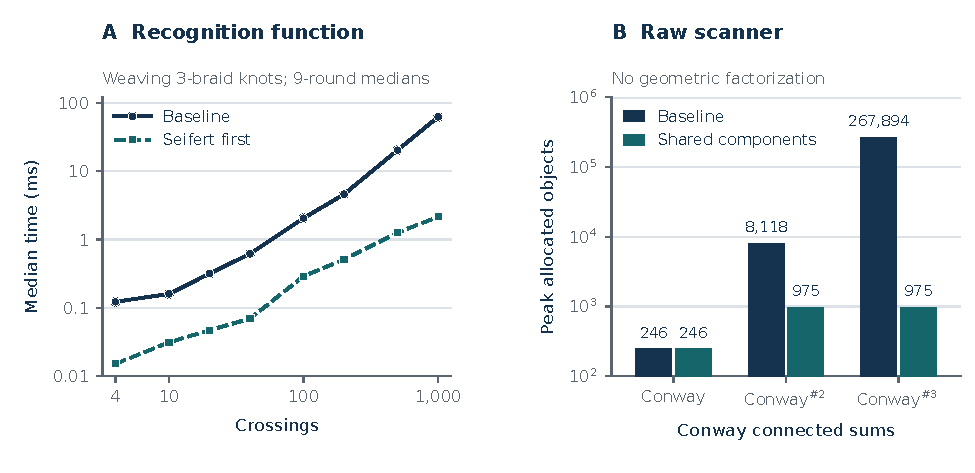
\includegraphics[width=\textwidth]{figures/performance_summary.pdf}
\caption{Two improvements with different measurement boundaries.
(A) Median recognition-function times on weaving three-strand knots in the
original structural experiment, nine rounds per input; parsing and validation
are excluded. Logarithmic axes and connecting segments show measurements,
with no fitted exponent. (B) Recorded maximum objects before elimination
in the raw baseline and exact shared scanners on one, two, and three Conway
summands, with geometric factorization disabled. These are scanner-object
counts, not process-memory measurements.}
\label{fig:performance}
\end{figure}

\subsection{Early Euler certificates}
The exact continuation recorder gives the following operation counts:
\begin{center}\small
\begin{tabular}{@{}lrrrr@{}}
\toprule
Input & Decision stage & Euler states & Scan $W$ at decision & Full shared $W$\\
\midrule
Two Conway summands & $11/22$ & 34 & 5,252 & 6,875\\
Three Conway summands & $11/33$ & 76 & 5,407 & 12,437\\
Eight Conway summands & $11/88$ & 286 & 5,252 & 39,317\\
\bottomrule
\end{tabular}
\end{center}
In each certificate the retained template has exact completed Euler
characteristic $+2$ and saturated multiplicity three. The resulting
nonnegative rank lower bound is capped at three and already exceeds the
unknot threshold. A one-state Euler budget on the eight-summand input
exhausts safely and completes the ordinary saturated scan at stage 88.

The Conway knot, stress braid, and hard-unknot controls trigger no Euler
states because they do not split early. The $T(3,5)$ example uses three
Euler states but yields no early verdict. It is a useful reminder that
nontrivial homology can have zero Euler characteristic within a summand.
The table counts Euler states separately: omitting their cost from $W$
must not be interpreted as omitting it from running time. No general
Euler-engine speedup is claimed from these diagnostic observations.

\subsection{What the evidence does and does not establish}
The structural front end changes the asymptotic cost of recognition on a
large, mathematically defined diagram class. The shared representations
remove an explicit multiplicity barrier and satisfy the finite-type theorem.
The Euler extension can use surviving summands as exact early witnesses.
All three are implemented and reproducibly tested.

The observed examples do not bound the sizes of future connected components,
prove a small frontier for arbitrary inputs, or certify that random tests
represent hard unknot diagrams. No fitted empirical exponent substitutes
for those missing structural statements. The default remains a complete
recognizer with an exponential worst-case upper bound, with \UNKNOWN\ under
optional resource ceilings. The following research programme addresses the
missing general theorem directly.

\section{The remaining route to general quasi-polynomial time}
\label{sec:route}

\subsection{Two routes with different missing theorems}
The current implementation can now avoid work in three distinct ways:
recognize a certified geometric class immediately; share repeated direct
summands; or prove sufficient final homology dimension from a partial scan.
None of these mechanisms gives a universal estimate on the frontier or on
the connected differential components.

The algebraic route needs a theorem that constructs a useful decomposition
of \emph{every} knot diagram, with controlled component complexity under
continuation. The hierarchy route needs an executable representation of
patterned handle structures, compressed surface operations, and a global
bound on effective restarts. These are different programmes. A successful
subroutine for one programme does not automatically discharge the other
programme's complexity obligations.

For the algebraic route, a quantitative target is to prove for some
constructively specified ordering or more general assembly rule that
\[
 b^2 2^{w/2}=O(\log^2 n).
\]
This target is sufficient rather than necessary. The type-count proof is
crude enough that a much sharper classification of reachable morphisms or
templates could replace it. It may be more realistic to control the number
of \emph{reachable} templates directly than to force every template to
have logarithmic size.

There is also a topological obstruction to reducing the frontier on every
input merely by choosing a better crossing order. The tree-width theorem
of de Mesmay, Purcell, Schleimer, and Sedgwick implies that every diagram
of a torus knot $T(p,q)$ has tree-width at least
$\min(p,q)/4-1$~\cite[Theorem 3.7]{treewidth}. A linear frontier scan
induces a carving decomposition up to constant factors, so the standard
$n=\Theta(p^2)$ diagrams of $T(p,p+1)$ require $w=\Omega(\sqrt n)$
under every such ordering. Their homogeneous structure is already handled
by the new front end. A useful general width theorem must therefore concern
the residual class after certificates, or a genuinely different
representation. Width of a knot diagram and width of a triangulated knot
complement must not be conflated; the same source shows that torus-knot
complements admit constant-tree-width triangulations.

\subsection{Nonuniform restart accounting for a future hierarchy engine}
The following elementary result is useful when different hierarchy levels
have substantially different complexity caps. It is stated independently of
any claim that the necessary geometric invariants have been implemented.

\begin{proposition}[Mixed-radix restart bound]\label{prop:radix}
Suppose an algorithm has a length-$L$ state vector
$(a_1,\ldots,a_L)$ with integer bounds $0\le a_i\le g_i$. At each restart,
the first changed coordinate strictly decreases; all subsequent coordinates
may reset arbitrarily within their fixed bounds. Then the number of such
restarts is at most
\[
 \prod_{i=1}^{L}(g_i+1)-1.
\]
If every between-restart operation has polynomial bit cost and all stored
encodings have polynomial size, a sufficient condition for the target
$n^{O(\log n)}$ is
\[
 \sum_{i=1}^{L}\log(g_i+1)=O(\log^2 n),
\]
with polynomially many operations between successive restarts.
\end{proposition}
\begin{proof}
Use the mixed-radix potential
\[
 \Phi(a_1,\ldots,a_L)=\sum_{i=1}^{L}a_i\prod_{j>i}(g_j+1).
\]
It is an integer between zero and $\prod_i(g_i+1)-1$. If coordinate $i$
is the first to change, decreasing it by one lowers $\Phi$ by
$\prod_{j>i}(g_j+1)$. The entire suffix can increase by at most that
quantity minus one. Every restart therefore decreases $\Phi$ by at least
one. Taking logarithms of the resulting product bound gives the last
statement after charging the polynomial overhead.
\end{proof}

The uniform case with $g_i=g$ gives the familiar $(g+1)^L$ factor. Polynomial
surface caps with $L=O(n)$ still permit $n^{O(n)}$ restarts. Polynomial caps
with $L=O(\log n)$ yield~\eqref{eq:target}; with
$L=O((\log n)^2)$ they give $2^{O((\log n)^3)}$. Coordinate compression
alone does not change this arithmetic.

The proposition is a template for a proof, not an observation that the
geometric algorithm already has this potential. The caps must be globally
valid after every reconstruction. A log recording decreasing numbers does
not establish either that validity or the topological correctness of the
restart operation.

\subsection{Concrete interface obligations for a hierarchy implementation}
The minimum coherent implementation unit is larger than a normal-coordinate
vector or a ball-pattern tester. It should include the following contracts.
\begin{enumerate}
\item \textbf{Encoded topology.} A finite list of allowed handle types, exact
attachment maps, boundary-pattern incidences, orientation, and an encoding
size charged to the input and all created objects.
\item \textbf{Compressed surface operations.} Binary multiplicities,
component and boundary information, cutting, gluing, and transport of curves
or discs across each change. A procedure must operate on binary size, rather
than expand one disc per unit of normal weight.
\item \textbf{Topology-preserving simplification.} Every parallelity-bundle
replacement or handle cleanup must carry a precise statement of the
manifold and boundary pattern it preserves or changes.
\item \textbf{Progress.} Surface production and violating-disc transport
must support a globally bounded potential through every replacement of a
hierarchy suffix, including changes to the representation itself.
\item \textbf{Cost composition.} Bound the number of generated handles,
coefficient lengths, calls, and restarts together. A fast primitive is
insufficient if called super-quasi-polynomially often.
\end{enumerate}
The Agol--Hass--Thurston orbit-count method is an established model for
processing exponentially long interval systems through short encodings
\cite{aht}. Its existence supports this design direction; it does not, by
itself, implement the full contracts above. The present archive leaves
these interfaces as a research programme rather than supplying placeholders
that report topological verdicts.

\section{Further research questions and proposed work}
\label{sec:questions}

The following questions are ordered by the strength and immediacy of the
connection to the delivered implementation. Each is paired with a concrete
success criterion.

\begin{enumerate}[label=\textbf{Q\arabic*.},leftmargin=*]
\item \textbf{Which prime families have bounded component size after sharing?}
Find an infinite family of prime, nonhomogeneous diagrams for which the
actual component-sharing policy has a proved bound on $b$ and $w$, and for
which earlier filters are not the entire explanation of fast recognition.
A proof must specify the scan order and the representative transition types.
A list of observed small components is useful evidence but not the result.

\item \textbf{Can reachable morphisms replace the all-masks bound?}
The factor $2^{s^2 2^{w/2}}$ counts every matrix entry in the full dot-mask
space. Identify a closure property of the entries actually produced by
extension and unit elimination. A bound on the number of reachable
coefficient masks could enlarge the quasi-polynomial regime substantially.
The proposed class must survive composition and Schur-complement addition.

\item \textbf{Can connected components be split efficiently after a basis
change?} The current graph decomposition finds literal blocks. Develop a
restricted, provably polynomial family of basis changes that reveals further
repeated summands. The output should include an explicit invertible change
of basis or chain-homotopy equivalence. A general canonical-form oracle
would merely move the hard computation elsewhere.

\item \textbf{How much can a pointed or reduced category expose?}
A carefully constructed marked-edge implementation might kill some
nonunit morphisms earlier and reveal smaller components. It must track the
basepoint through all gluing and delooping operations, prove compatibility
with reduced homology, and preserve a finite composition algebra. This
archive does not include an unverified quotient obtained by simply deleting
dot terms touching a chosen boundary point.

\item \textbf{Can continuation-aware obstructions be strengthened?}
Theorem~\ref{thm:euler} uses one scalar Euler functional for each completed
summand. Investigate several quantum-graded evaluations or other additive
functionals with certified norm bounds. The central requirement is a proved
lower bound on homology rank after continuation. Capping signed sums before
cancellation would invalidate such a certificate.

\item \textbf{When should the optional Euler engine run?}
Develop a predictor based on cheap component statistics or a small number
of exact suffix values. Measure total time including failed inference.
Any adaptive policy must preserve the property that a budget failure simply
returns to a complete backend. Establishing a profitable policy on prime
filter-resistant diagrams would be more informative than optimizing the
visible-sum stress family again.

\item \textbf{Can a complete three-braid rank engine be integrated?}
The polynomial-time three-braid result in the 2026 literature suggests a
specialized exact backend based on normal forms and formulas
\cite{kelomaki}. Implementation requires careful grading, mirror, linking,
and coefficient conventions. Validate it against the independent cube and
both scanning algebras before using it to bypass scanning. The mere fact
that the input has three strands is not a complexity theorem for the
current scanner.

\item \textbf{Can extremal-band complexity be made uniform?}
Seek a fully quantified finite-field bound such as
$2^{O(w)}n^{O(k)}$ for computing a band of $k$ homological degrees under an
explicitly specified assembly rule. The number of objects, decorated
morphisms, coefficient sizes, and the extra degree needed for outgoing
differentials must all be charged. A complete recognizer would still need a
proved location of a nontriviality witness in those bands or a fallback.

\item \textbf{What structural parameter survives reduction?}
Example~\ref{ex:defectone} and the I/II-reduced family in
Section~\ref{sec:reduced-defect-one} rule out control by homogeneity defect
alone. Search for a parameter combining signed block structure with a
certified diagram reduction or tangle decomposition. It should distinguish
many redundant twists from genuine mixed-sign complexity.

\item \textbf{Can a controlled portfolio improve the heavy tail?}
Sharing, saturated sharing, Euler inference, the ordinary scanner, and
geometric reduction have different overheads. A portfolio should be judged
by CPU work as well as wall time. A useful guarantee would compare its cost
with the best applicable complete backend, while bounding the work lost in
abandoned runs. Purely retrospective selection of the fastest run is not an
implementable performance claim.

\item \textbf{Can the new proof obligations be formalized?}
A small formal development can first prove the $S_3$ semiring quotient,
weighted direct-sum transition invariant, and monotone Euler bound. These
have explicit finite algebraic interfaces. Formalizing the full
Bar-Natan category and the unknot-detection theorem is a separate,
substantially larger task. A checked combinatorial certificate still depends
on its imported topological soundness theorem.

\item \textbf{Can the hierarchy route obtain a nonuniform progress bound?}
Implement a complete unaccelerated hierarchy engine with explicit contracts,
then search for level-dependent caps satisfying
Proposition~\ref{prop:radix}. A successful result would specify the caps,
the retained suffix under each simplification, and the proof that every
expensive restart is counted. This is a direct path to a real end-to-end
quasi-polynomial theorem, but it remains beyond the delivered changes.
\end{enumerate}

\section{Concluding assessment}
The delivered recognizer has a broader polynomially decidable front end and
an exact mechanism for representing repeated chain-complex summands without
expanding their generators. Saturated weights specialize that representation
to the actual yes/no problem, and exact Euler continuations supply a safe
form of early nontriviality detection. The finite-type theorem identifies a
specific sufficient regime for $n^{O(\log n)}$ time that accounts for both
algebraic state size and integer arithmetic.

The implementation retains an exponential worst-case upper bound; no general
quasi-polynomial bound is proved. The
measured improvement on homogeneous families is an end-to-end pipeline
improvement after validation. The dramatic connected-sum scanner figures
are representation stress tests, because an earlier specialized factorizer
already handles those examples efficiently. The hardest remaining task is
to control structural complexity for diagrams that are neither certified by
the front end nor decomposed into small repeated components. The archive
provides an executable basis for pursuing that task and exact criteria for
judging whether a future claim has actually reached the quasi-polynomial
target.

% Bibliographic records and theorem locators checked against primary papers,
% author pages, and publisher records on 7 October 2026.
% The bibliography is self-contained: no BibTeX/Biber invocation is needed.
\begin{thebibliography}{99}
\addcontentsline{toc}{section}{References}

\bibitem{abe}
Tetsuya Abe,
\emph{The Rasmussen invariant of a homogeneous knot},
Proceedings of the American Mathematical Society
\textbf{139} (2011), no.~7, 2647--2656.
\href{https://doi.org/10.1090/S0002-9939-2010-10687-1}{doi:10.1090/S0002-9939-2010-10687-1}.
\href{https://arxiv.org/abs/1003.5392}{arXiv:1003.5392}.
Theorems~2.3 and~3.4 give the genus statement and homogeneity criterion used here.

\bibitem{aht}
Ian Agol, Joel Hass, and William P.~Thurston,
\emph{The computational complexity of knot genus and spanning area},
Transactions of the American Mathematical Society
\textbf{358} (2006), no.~9, 3821--3850.
\href{https://doi.org/10.1090/S0002-9947-05-03919-X}{doi:10.1090/S0002-9947-05-03919-X}.
\href{https://arxiv.org/abs/math/0205057v2}{arXiv:math/0205057v2}.
Theorems~12 and~16 describe ordinary and weighted orbit counting.

\bibitem{weaving}
Mark E.~AlSukaiti and Nafaa Chbili,
\emph{Alexander and Jones polynomials of weaving 3-braid links and Whitney
rank polynomials of Lucas lattice},
Heliyon \textbf{10} (2024), no.~7, article e28945.
\href{https://doi.org/10.1016/j.heliyon.2024.e28945}{doi:10.1016/j.heliyon.2024.e28945}.
\href{https://arxiv.org/abs/2303.11398}{arXiv:2303.11398}.
See Corollary~3.5 of the arXiv version for the determinant formula.

\bibitem{bnfast}
Dror Bar-Natan,
\emph{Fast Khovanov homology computations},
Journal of Knot Theory and Its Ramifications
\textbf{16} (2007), no.~3, 243--255.
\href{https://doi.org/10.1142/S0218216507005294}{doi:10.1142/S0218216507005294}.
\href{https://arxiv.org/abs/math/0606318}{arXiv:math/0606318}.
\href{https://www.math.toronto.edu/drorbn/papers/FastKh/FastKh.pdf}{Author's version of 20 May 2007}.

\bibitem{cromwell}
Peter R.~Cromwell,
\emph{Homogeneous links},
Journal of the London Mathematical Society (2)
\textbf{39} (1989), no.~3, 535--552.
\href{https://doi.org/10.1112/jlms/s2-39.3.535}{doi:10.1112/jlms/s2-39.3.535}.

\bibitem{treewidth}
Arnaud de~Mesmay, Jessica Purcell, Saul Schleimer, and Eric Sedgwick,
\emph{On the tree-width of knot diagrams},
Journal of Computational Geometry
\textbf{10} (2019), no.~1, 164--180.
\href{https://doi.org/10.20382/jocg.v10i1a6}{doi:10.20382/jocg.v10i1a6}.
\href{https://arxiv.org/abs/1809.02172v2}{arXiv:1809.02172v2}.
See Theorem~3.7 and Corollary~1.2 for the obstruction to uniformly small
diagrammatic tree-width.

\bibitem{kelomaki}
Tuomas Kelom\"aki and Dirk Sch\"utz,
\emph{On computational complexity of Khovanov homology},
preprint, 5 January 2026, 30~pp.
\href{https://arxiv.org/abs/2601.02119v1}{arXiv:2601.02119v1}.
Theorems~1.2--1.4 distinguish the explicit-basis obstruction,
the specialized three-braid algorithm, and extremal homological bands.

\bibitem{km}
Peter B.~Kronheimer and Tomasz S.~Mrowka,
\emph{Khovanov homology is an unknot-detector},
Publications Math\'ematiques de l'IH\'ES
\textbf{113} (2011), 97--208.
\href{https://doi.org/10.1007/s10240-010-0030-y}{doi:10.1007/s10240-010-0030-y}.
\href{https://arxiv.org/abs/1005.4346}{arXiv:1005.4346}.
The rational-rank implication used here follows from Corollary~1.3,
Proposition~1.4, and the unknot detection discussed in the introduction.

\bibitem{lackenbytalk}
Marc Lackenby,
\emph{Unknot recognition in quasi-polynomial time},
Oxford topology seminar handout, March 2021, 34~pp.
\url{https://people.maths.ox.ac.uk/lackenby/quasipolynomial-talk-oxford-compressed.pdf}.
The announced bound is displayed on slide~7; the four proposed speed-ups
are summarized on slide~25.

\bibitem{lackenby2026}
Marc Lackenby,
\emph{Incompressible surfaces, hierarchies and unknot recognition},
preprint, 25 July 2026, 54~pp.
\href{https://arxiv.org/abs/2607.23350v1}{arXiv:2607.23350v1}.
\href{https://people.maths.ox.ac.uk/lackenby/algorithm-incompressible-250726.pdf}{Author's PDF}.
See Propositions~9.1 and~10.2 for the iteration and hierarchy-length bounds,
and Theorem~14.4 for compressed cutting under uniform-type hypotheses.

\bibitem{lobb}
Andrew Lobb,
\emph{Computable bounds for Rasmussen's concordance invariant},
Compositio Mathematica
\textbf{147} (2011), no.~2, 661--668.
\href{https://doi.org/10.1112/S0010437X10005117}{doi:10.1112/S0010437X10005117}.
\href{https://arxiv.org/abs/0908.2745v2}{arXiv:0908.2745v2}.
The interval used here is Theorem~1.10, with Definitions~1.8--1.9.

\bibitem{manchon}
Pedro M.~G.~Manch\'on,
\emph{Homogeneous links and the Seifert matrix},
Pacific Journal of Mathematics
\textbf{255} (2012), no.~2, 373--392.
\href{https://doi.org/10.2140/pjm.2012.255.373}{doi:10.2140/pjm.2012.255.373}.
\href{https://arxiv.org/abs/1102.0890v2}{arXiv:1102.0890v2}.

\bibitem{morton}
Hugh R.~Morton,
\emph{The multivariable Alexander polynomial for a closed braid},
in \emph{Low-dimensional topology} (Funchal, 1998),
Hanna Nencka, ed., Contemporary Mathematics \textbf{233},
American Mathematical Society, Providence, RI, 1999, 167--172.
\href{https://arxiv.org/abs/math/9803138}{arXiv:math/9803138}.
The introduction and the discussion following Theorem~1 state the
reduced Burau closure formula.

\bibitem{proveit}
Vladimir Reshetnikov,
\emph{ProveIt: Topology/UnknotRecognition},
software and research repository, source snapshot at commit
\pin, accessed 7 October 2026.
\url{https://github.com/VladimirReshetnikov/ProveIt/tree/4e6fe879e5238ec0b134b6d33fdca0b8c7c1c711/Topology/UnknotRecognition}.

\bibitem{shumakovitch}
Alexander N.~Shumakovitch,
\emph{Torsion of Khovanov homology},
Fundamenta Mathematicae \textbf{225} (2014), 343--364.
\href{https://doi.org/10.4064/fm225-1-16}{doi:10.4064/fm225-1-16}.
\href{https://arxiv.org/abs/math/0405474v2}{arXiv:math/0405474v2}
(updated 19 June 2018 to match the published version; arXiv title:
\emph{Torsion of the Khovanov homology}).
Corollary~3.2.C, on published page~356, gives the reduced/unreduced
splitting over $\mathbb F_2$.

\end{thebibliography}

\end{document}
